\chapter{劉維爾定理與哈密頓流}

\lectureoverview{哈密頓方程所做的遠不只是重新表述運動方程。它們在相空間上定義了一個散度為零的速度場。這個簡單的相消就是劉維爾定理：哈密頓演化會保持相空間體積。我們將依照其物理意義逐步顯現的順序推導這個定理---：先談能量守恆，再談等能面，接著把可能的初始條件視為流體，最後比較保體積流與耗散匯。同樣的語言也自然引出泊松括號。}

\section{為什麼還需要另一種力學形式？}

我們要討論的定理，是課程一開始介紹的可逆狀態圖在連續經典系統中的對應。在可逆的離散定律中，每個狀態都有一個箭頭進入，也有一個箭頭離開。現在的狀態足以決定下一個狀態和前一個狀態。若定律不理想，許多狀態會流入同一個匯：未來或許仍可確定，但過去已無法還原。

劉維爾定理說明，當狀態集合是連續相空間時，這種差異會如何呈現。取代「一個箭頭進入、一個箭頭離開」的說法，將是\emph{流入量等於流出量}。然而，要讓這句話成為數學陳述，我們得先從哈密頓方程重建這個流。

重建的過程有一個歷史上的謎題。哈密頓、雅可比、拉格朗日和泊松發展出精巧而優美的經典力學形式，卻不知道量子理論日後會使這些形式變得不可或缺。牛頓有一個直接的目標：行星運動。拉格朗日和哈密頓也面對具體的物理問題，但他們追求的類比與結構遠超出任何單一軌道。力學中的定常作用量原理，與光學中的最短時間原理相似；光線運動和粒子運動可以用平行的數學形式描述。他們簡化、重整並統一方程，是因為這些結構本身似乎就蘊含著物理。

我們現在知道，這種直覺帶來了非凡的成果。從邏輯上看，經典力學的許多特徵可以理解為量子力學的極限。但歷史發展的順序正好相反：經典結構先被發現，直到很久以後，人們才看清它們更深層的用途。一則歸於費曼的挑釁性笑話，以數學在自身內部的探索，對比受外在夥伴——物理世界——約束的物理學，來表達這一點。這則笑話不是論證，但這個區別很有啟發性：形式之美在此之所以重要，是因為自然界一再採用這些形式結構。

\begin{classroomqa}
  \audiencequestion{牛頓是否具備現代的動能概念？能量這個概念又是從何時開始的？
  \lecturetimestamp{00:04:24--00:05:50}}
  \lecturerresponse{牛頓力學以力和運動為核心，尚未建立成熟的一般能量原理。這段討論並未判定能量概念確切的歷史優先權。萊布尼茲的\emph{活力}，\(\sum_i m_i v_i^2\)，是重要的前身，數值等於現代動能的兩倍。後來對熱的研究，使熱與機械功之間的轉換成為核心議題。早期的熱質說把熱視為一種守恆物質，因此，能量可以不同形式相互轉換的現代觀念，是逐漸形成的。}
\end{classroomqa}

\section{哈密頓方程與能量守恆}

設系統有\(n\)對正則變數，
\begin{equation}
  (q_i,p_i),\qquad i=1,\ldots,n.
  \label{eq:l7-canonical-pairs}
\end{equation}
每個座標各有一個動量，每個動量也各有一個座標。運動定律由一個函數統一表示，
\begin{equation}
  H=H(q_1,\ldots,q_n,p_1,\ldots,p_n,t),
  \label{eq:l7-hamiltonian}
\end{equation}
而哈密頓方程為
\begin{equation}
  \boxed{
  \dot q_i=\frac{\partial H}{\partial p_i},
  \qquad
  \dot p_i=-\frac{\partial H}{\partial q_i}.}
  \label{eq:l7-hamilton-equations}
\end{equation}
正負號是正則結構的一部分。\(q\)方程帶正號；\(p\)方程帶負號。

\begin{figure}[htbp]
  \centering
  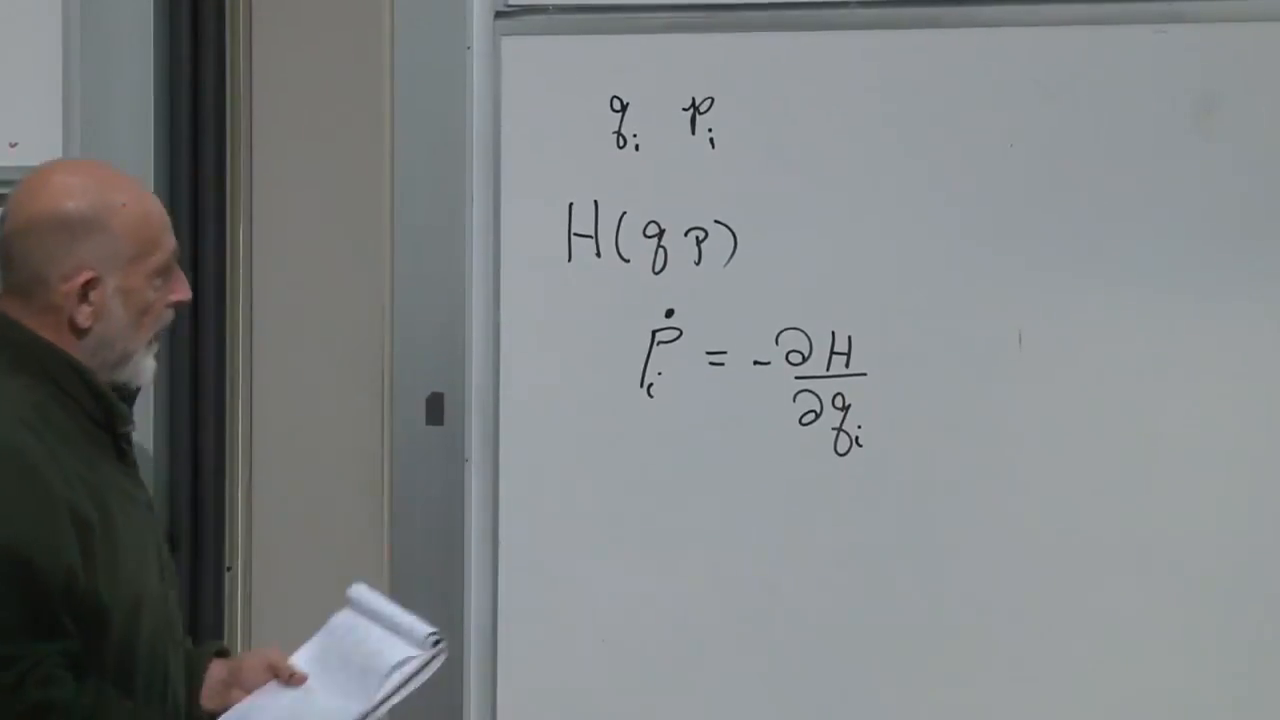
\includegraphics[width=0.82\textwidth]{lecture_07_figure_02.png}
  \caption{正則變數、函數\(H(q,p)\)，以及回顧一開始所列的動量側哈密頓方程。}
  \lectureframe{00:07:29}
\end{figure}

雖然方程以成對的指標形式出現，動力學不一定會逐對分離。哈密頓量可能耦合所有的\(q_i\)和\(p_i\)，因此，例如\(\dot p_1\)可能取決於整個系統的狀態。

\begin{classroomqa}
  \audiencequestion{這種表述現在是公理化的嗎？\(p\)和\(q\)之間假設了什麼關係？
  \lecturetimestamp{00:17:08--00:18:18}}
  \lecturerresponse{指定\(H(q,p)\)和正則變數對之後，哈密頓方程就定義了形式理論。並沒有普遍適用的額外假設\(p=m\dot q\)。對於動能為二次形式的普通笛卡兒粒子，這個關係成立；但採用其他座標或其他哈密頓量時，動量--速度關係也會不同。方程本身透過\(\dot q_i=\partial H/\partial p_i\)給出這個關係。至於提出的哈密頓量是否在自然界中實現，則是另一個物理問題。}
\end{classroomqa}

現在只需一步推理，就能得到能量守恆。沿著一條軌跡，\(H\)的全導數為
\begin{equation}
  \frac{dH}{dt}
  =
  \sum_i\left(
    \frac{\partial H}{\partial q_i}\dot q_i
    +\frac{\partial H}{\partial p_i}\dot p_i
  \right)
  +\frac{\partial H}{\partial t}.
  \label{eq:l7-total-h-derivative}
\end{equation}
最後一項表示\(q\)和\(p\)固定時仍存在的顯式時間依賴，例如外部指定的參數正在變化。代入式~\eqref{eq:l7-hamilton-equations}，
\begin{align}
  \frac{dH}{dt}
  &=
  \sum_i\left[
    \frac{\partial H}{\partial q_i}
    \frac{\partial H}{\partial p_i}
    -\frac{\partial H}{\partial p_i}
    \frac{\partial H}{\partial q_i}
  \right]
  +\frac{\partial H}{\partial t}\\
  &=\frac{\partial H}{\partial t}.
  \label{eq:l7-h-energy-rate}
\end{align}
總和中的每一項都會和配對項相消。因此，
\begin{equation}
  \frac{\partial H}{\partial t}=0
  \quad\Longrightarrow\quad
  \frac{dH}{dt}=0.
  \label{eq:l7-energy-conservation}
\end{equation}
對於封閉且具有時間平移不變性的系統，哈密頓量守恆，而且就是能量。

\begin{classroomqa}
  \audiencequestion{如果哈密頓量顯式依賴時間，會有什麼變化？\lecturetimestamp{00:10:32--00:12:33}}
  \lecturerresponse{式~\eqref{eq:l7-h-energy-rate}仍然成立，但子系統的能量不一定保持定值。顯式時間依賴通常表示有一個未納入模型的驅動源正在與系統交換能量。如果將這個驅動源納入更大的封閉系統，使它也成為動力學的一部分，那麼較大系統的哈密頓量便可再次不隨時間改變，總能量也會守恆。}
\end{classroomqa}

\section{相空間中的能量幾何}

現在假設\(H\)沒有顯式時間依賴。初始條件決定一個數值\(E\)，而相點會一直留在
\begin{equation}
  H(q,p)=E.
  \label{eq:l7-energy-surface}
\end{equation}
相空間有\(2n\)維。在正則點上，一個座標方程會定義一個\((2n-1)\)維超曲面。不同的\(E\)值會給出不同的超曲面。這些超曲面不一定封閉或緊緻；能量守恆只表示，從其中一個超曲面出發的軌跡永遠不會離開它。

對於前一講中經過適當縮放的諧振子，
\begin{equation}
  H=\frac{\omega}{2}(p^2+q^2).
  \label{eq:l7-oscillator-hamiltonian}
\end{equation}
因此，每個等能集合都是一個圓，
\begin{equation}
  p^2+q^2=\frac{2E}{\omega}.
  \label{eq:l7-oscillator-circle}
\end{equation}

\begin{figure}[htbp]
  \centering
  \includegraphics[width=0.84\textwidth]{lecture_07_figure_04.png}
  \caption{\(2n\)維相空間示意圖，以及用來引入等能面的諧振子哈密頓量。}
  \lectureframe{00:15:20}
\end{figure}

運動方程
\begin{equation}
  \dot q=\omega p,\qquad \dot p=-\omega q,
  \label{eq:l7-oscillator-flow}
\end{equation}
使相點沿著圓順時針運動。能量方程指出運動所在的曲線；哈密頓方程則給出沿著該曲線運動的方向和速率。

\begin{figure}[htbp]
  \centering
  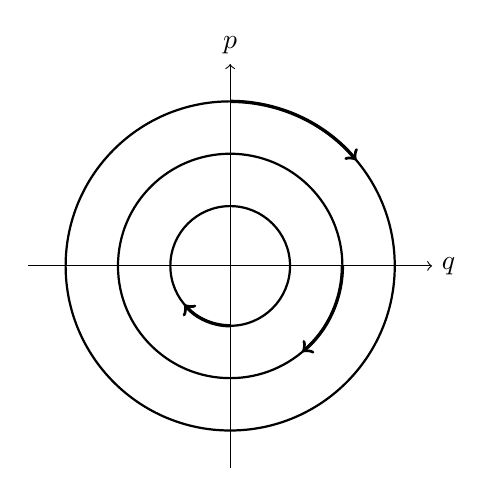
\begin{tikzpicture}[scale=0.95]
    \draw[->] (-2.7,0) -- (2.7,0) node[right] {\(q\)};
    \draw[->] (0,-2.7) -- (0,2.7) node[above] {\(p\)};
    \draw[thick] (0,0) circle (0.8);
    \draw[thick] (0,0) circle (1.5);
    \draw[thick] (0,0) circle (2.2);
    \draw[->,very thick] (0,2.2) arc[start angle=90,end angle=40,radius=2.2];
    \draw[->,very thick] (1.5,0) arc[start angle=0,end angle=-50,radius=1.5];
    \draw[->,very thick] (0,-0.8) arc[start angle=-90,end angle=-140,radius=0.8];
  \end{tikzpicture}
  \caption{等能條件決定這些圓；振子方程則給出順時針的切向流。}
\end{figure}

\begin{classroomqa}
  \audiencequestion{哈密頓的兩個方程和\(H=E\)，是同一個方程的不同形式嗎？
  \lecturetimestamp{00:15:53--00:17:06}}
  \lecturerresponse{不是。哈密頓方程是描述一組正則變數對的兩條一階運動定律。它們蘊含\(dH/dt=0\)，由此可推出\(H=E\)。\(E\)的值由初始條件決定。方程\(H=E\)指出一個曲面，但本身不會指定沿著該曲面的速度。}
\end{classroomqa}

\section{從單一狀態到狀態流}

與其追蹤一個初始條件，不如讓相空間布滿所有可能的初始條件，再啟動時鐘。每個點代表一個完整的可能狀態，而每個狀態都依照哈密頓方程演化。我們可以把這些點想像成塵埃或假想流體。沒有任何物質真的被倒進相空間；流體只是讓我們能同時觀察所有軌跡的一種想像方式。

相空間中的速度場為
\begin{equation}
  \mathbf V(q,p,t)
  =
  (\dot q_1,\ldots,\dot q_n,\dot p_1,\ldots,\dot p_n).
  \label{eq:l7-phase-velocity}
\end{equation}
對於一組正則變數，我們寫成
\begin{equation}
  V_q=\dot q=\frac{\partial H}{\partial p},
  \qquad
  V_p=\dot p=-\frac{\partial H}{\partial q}.
  \label{eq:l7-phase-components}
\end{equation}
在每一點，哈密頓量都指定一個向量，表示相點接下來的運動方向。如果\(H\)不隨時間變化，向量場就是定常的：回到同一個相點時，速度仍相同。如果\(H\)依賴時間，向量場本身會隨時間改變，但在每一瞬間仍有明確定義。

\begin{figure}[htbp]
  \centering
  \includegraphics[width=0.84\textwidth]{lecture_07_figure_05.png}
  \caption{諧振子的速度場。向量沿圓的切線方向，且越接近原點，向量越短。}
  \lectureframe{00:24:50}
\end{figure}

對諧振子而言，每個半徑都以角速度\(\omega\)轉動。靠近原點的點，其線速度較小，因為它們在相同週期內走過的圓周較短。因此，整團塵埃會像剛體旋轉般轉動。

\begin{classroomqa}
  \audiencequestion{剛體般旋轉是否表示所有諧振子軌跡的週期都相同？\lecturetimestamp{00:21:10--00:21:42}}
  \lecturerresponse{是。週期與振幅無關，正是諧振子的特有性質。每個圓都以相同的角頻率\(\omega\)繞行，儘管較小圓上的相空間速度量值較小。}
\end{classroomqa}

\begin{classroomqa}
  \audiencequestion{相空間速度在每一點都相同嗎？
  \lecturetimestamp{00:24:29--00:25:37}}
  \lecturerresponse{不是。速度的方向和量值通常都會隨位置改變。對諧振子而言，向量沿著當地圓的切線方向，量值為\(\omega\sqrt{p^2+q^2}\)。所謂向量場，是指每一點各有一個向量，而不是把同一個向量複製到每個位置。}
\end{classroomqa}

\begin{classroomqa}
  \audiencequestion{這種假想流體中的粒子和密度，究竟代表什麼？\lecturetimestamp{00:56:03--00:58:40}}
  \lecturerresponse{每一個點代表整個力學系統的一個完整狀態，並非一個物理粒子。五個粒子在一維空間中運動，需要五個位置和五個動量，因此相空間有十個維度；若是在三維空間中，則需要三十個維度。這團塵埃代表一組彼此替代的可能狀態。如果流體圖像令人分心，只要取一個初始條件區域，讓其中每一點演化，再比較演化前後的相空間體積即可。}
\end{classroomqa}

\section{壓縮與散度}

要判斷這種假想流體是否會失去體積，先從一維開始。設直線上的點以速度\(v(x)\)運動。兩個相距\(\delta x\)的鄰近點，其速度差為
\begin{equation}
  \delta v \simeq \frac{dv}{dx}\,\delta x.
  \label{eq:l7-one-dimensional-strain}
\end{equation}
若\(dv/dx>0\)，前方的點移動得較快，兩點間隔便會拉長。若\(dv/dx<0\)，間隔便會壓縮。因此，定常的一維不可壓縮流必須滿足
\begin{equation}
  \frac{dv}{dx}=0.
  \label{eq:l7-one-dimensional-incompressible}
\end{equation}

\begin{figure}[htbp]
  \centering
  \includegraphics[width=0.84\textwidth]{lecture_07_figure_06.png}
  \caption{一維推導：\(dv/dx\)是局部拉伸或壓縮的速率。}
  \lectureframe{00:30:20}
\end{figure}

有兩種等價的觀點。我們可以跟著一段流體移動，觀察它的長度是否改變；也可以固定一個小區間，觀察單位時間內流入的量是否等於流出的量。前者跟著流體走，後者觀察流體經過。

在多維空間中，一個區域可以沿某個軸拉伸，同時沿另一個軸壓縮，而總體積仍不變。對於速度場\(\mathbf V=(V_x,V_y,V_z)\)，相關的局部速率是散度：
\begin{equation}
  \nabla\cdot\mathbf V
  =
  \frac{\partial V_x}{\partial x}
  +\frac{\partial V_y}{\partial y}
  +\frac{\partial V_z}{\partial z}.
  \label{eq:l7-spatial-divergence}
\end{equation}
散度為正表示局部膨脹，散度為負表示局部收縮；不可壓縮條件則是
\begin{equation}
  \nabla\cdot\mathbf V=0.
  \label{eq:l7-zero-divergence}
\end{equation}
固定小盒的流入量等於流出量，與隨流動移動的小盒體積保持不變，是同一個局部陳述。

\begin{figure}[htbp]
  \centering
  \includegraphics[width=0.86\textwidth]{lecture_07_figure_07.png}
  \caption{二維小盒、流速分量，以及定義散度的同座標偏導數之和。}
  \lectureframe{00:35:30}
\end{figure}

\begin{classroomqa}
  \audiencequestion{我們談的是普通空間中的流體，還是相空間中的流？ \lecturetimestamp{00:34:27--00:34:40}}
  \lecturerresponse{散度的推導首先是一般的流體力學論證。我們會將它應用於偶數維的相空間；其中的座標方向是\(q_i\)和\(p_i\)，速度分量則是\(\dot q_i\)和\(\dot p_i\)。}
\end{classroomqa}

現在回到離散狀態映射。在可逆循環中，每個節點都有一個箭頭進入，也有一個箭頭離開；一組選定的狀態在演化後仍包含相同數量的狀態。在匯中，進入的箭頭很多，離開的箭頭卻太少；幾種不同的可能狀態因此變得無法區分。

\begin{figure}[htbp]
  \centering
  \includegraphics[width=0.80\textwidth]{lecture_07_figure_08.png}
  \caption{離散匯的示意圖，用來重新連結散度與第一講中檢驗定律可逆性的方式。}
  \lectureframe{00:40:15}
\end{figure}

現在可以精確地提出連續情況下的問題：哈密頓流的散度是否為零，因此一小塊可區分狀態的區域不會被壓縮成更小的相空間體積？

\section{劉維爾定理}

\begin{theorem}[Liouville's theorem]對於光滑的哈密頓系統，正則相空間中的速度場散度為零：
\begin{equation}
  \sum_i\left(
    \frac{\partial\dot q_i}{\partial q_i}
    +\frac{\partial\dot p_i}{\partial p_i}
  \right)=0.
  \label{eq:l7-liouville-divergence}
\end{equation}
等價地說，哈密頓演化會保持正則相空間體積\(dq_1\cdots dq_n\,dp_1\cdots dp_n\)。
\end{theorem}

\begin{classroomqa}
  \audiencequestion{稱為\(V\)的分量，就是\(p\)點和\(q\)點嗎？\lecturetimestamp{00:42:20--00:43:22}}
  \lecturerresponse{是。對於一組正則變數，
  \(V_q=\dot q\)和\(V_p=\dot p\)。將所有這類導數依序排列，就得到完整相空間中流動的速度向量。}
\end{classroomqa}

對於一組正則變數，哈密頓方程給出
\begin{equation}
  V_p=-\frac{\partial H}{\partial q},
  \qquad
  V_q=\frac{\partial H}{\partial p}.
  \label{eq:l7-liouville-components}
\end{equation}
因此散度為
\begin{align}
  \frac{\partial V_p}{\partial p}
  +\frac{\partial V_q}{\partial q}
  &=
  -\frac{\partial}{\partial p}
    \left(\frac{\partial H}{\partial q}\right)
  +\frac{\partial}{\partial q}
    \left(\frac{\partial H}{\partial p}\right)\\
  &=
  -\frac{\partial^2H}{\partial p\,\partial q}
  +\frac{\partial^2H}{\partial q\,\partial p}
  =0.
  \label{eq:l7-liouville-proof}
\end{align}

\begin{figure}[htbp]
  \centering
  \includegraphics[width=0.86\textwidth]{lecture_07_figure_09.png}
  \caption{有限差分矩形示意圖，用來說明光滑函數的混合偏導數為何可以交換次序。}
  \lectureframe{00:47:30}
\end{figure}

取\(A,B,C,D\)這四個點，分別位於\(q\)-\(p\)平面上一個小矩形的四個角，就能看出混合偏導數相等。先對\(q\)取差分，再對\(p\)取差分，除去兩條小邊的長度後，得到
\begin{equation}
  F(B)+F(D)-F(A)-F(C).
  \label{eq:l7-finite-difference-combination}
\end{equation}
若以相反次序取差分，也會得到相同的組合。在小矩形極限下，只要所需的導數連續，便有
\(\partial_p\partial_qF=\partial_q\partial_pF\)。

\begin{figure}[htbp]
  \centering
  \includegraphics[width=0.88\textwidth]{lecture_07_figure_10.png}
  \caption{哈密頓方程將正則散度化為兩個符號相反的混合偏導數。}
  \lectureframe{00:50:20}
\end{figure}

對於多個自由度，每一組正則變數都會發生相同的相消：
\begin{align}
  \sum_i\left(
    \frac{\partial\dot p_i}{\partial p_i}
    +\frac{\partial\dot q_i}{\partial q_i}
  \right)
  &=
  \sum_i\left(
    -\frac{\partial^2H}{\partial p_i\,\partial q_i}
    +\frac{\partial^2H}{\partial q_i\,\partial p_i}
  \right)\\
  &=0.
  \label{eq:l7-many-pair-proof}
\end{align}
沿一個正則方向的拉伸，會由其共軛方向的壓縮抵銷。這種逐對相消具有更深的結構，並非彼此無關的座標軸之間偶然相消。

\begin{classroomqa}
  \audiencequestion{這裡是否省略了對所有正則變數對求和？
  \lecturetimestamp{00:52:00--00:52:36}}
  \lecturerresponse{是。式~\eqref{eq:l7-many-pair-proof}是對\(i\)求和，而且每一組\(q_i,p_i\)變數對中的兩個混合偏導數都各自相消。}
\end{classroomqa}

\begin{classroomqa}
  \audiencequestion{寫出的散度看起來是笛卡兒座標形式。換了座標之後，定理還成立嗎？
  \lecturetimestamp{00:52:50--00:53:22,\allowbreak\ 00:58:18--00:58:40}}
  \lecturerresponse{自然的表述採用正則座標和正則體積元素\(dq_1\cdots dq_n\,dp_1\cdots dp_n\)。正則變換又稱辛變換，它會同時改變座標與動量，並保持這個體積。在任意非正則座標中，體積測度必須包含雅可比因子；座標增量的直接乘積不一定是不變量。}
\end{classroomqa}

\begin{classroomqa}
  \audiencequestion{劉維爾定理是否要求哈密頓量不隨時間變化？\lecturetimestamp{00:53:43--00:55:51}}
  \lecturerresponse{不要求。能量守恆需要\(\partial H/\partial t=0\)，但散度的推導只在固定時間下對\(q_i\)和\(p_i\)微分。對於\(H(q,p,t)\)，混合偏導數仍然會相消。因此，含時哈密頓量會產生隨時間變化、但每一瞬間都保持體積的正則流。}
\end{classroomqa}

\section{體積保持意味著什麼，又不意味著什麼}

取一個初始條件的小區域\(R_0\)，讓其中每個點演化時間\(t\)。劉維爾定理指出
\begin{equation}
  \operatorname{Vol}(R_t)=\operatorname{Vol}(R_0).
  \label{eq:l7-volume-preservation}
\end{equation}
這個區域可能移動、旋轉、剪切，並拉伸成細長的絲狀結構。受到保護的是體積，而不是形狀。在有限時間的光滑哈密頓演化中，不同的相點不會合併。

在有限時間內，光滑的哈密頓流是可逆映射；其光滑逆映射可藉由反向演化得到。這也說明了課堂上的說法：一團連通區域不會被掐斷成不連通的部分。流會連續地形變這個區域並保持其拓撲；不過，極細的連接頸部可能讓兩個瓣在有限解析度下看起來像是分開的。

\begin{figure}[htbp]
  \centering
  \includegraphics[width=0.86\textwidth]{lecture_07_figure_12.png}
  \caption{相空間區域可能發生的形變。光滑的哈密頓流可以形成細長的頸部，但不會在有限時間內真正斷裂成各自獨立演化的部分。}
  \lectureframe{01:04:55}
\end{figure}

\begin{classroomqa}
  \audiencequestion{相空間中的一個區域能否被掐斷，分裂成兩部分？\lecturetimestamp{01:04:10--01:05:49}}
  \lecturerresponse{在有限時間的光滑確定性哈密頓流下不會。即使在假想的掐斷點上，那仍是一個相點，只對應一個指定速度，而不會有兩個互不相容的方向。這個區域可以形成非常長而狹窄的連接細絲，但演化仍是一對一的，不會把它撕裂。}
\end{classroomqa}

\begin{classroomqa}
  \audiencequestion{被拉伸的區域中，兩個相距很遠的瓣在物理上仍相連嗎？它們是否量子糾纏？
  \lecturetimestamp{01:08:01--01:09:16}}
  \lecturerresponse{這並不表示它們在物理上相連。這個區域代表一組可能的初始條件，而不是一個物質物體。稱它為同一個區域，只是表示這些狀態源自同一個集合；這並不表示它們彼此間存在作用力或量子糾纏。}
\end{classroomqa}

\begin{classroomqa}
  \audiencequestion{剛性擺在鉛直向上的不穩定平衡附近會發生什麼事？順時針和逆時針的軌跡會重疊嗎？
  \lecturetimestamp{01:07:07--01:07:47}}
  \lecturerresponse{鄰近的初始條件可能分別沿著差異極大的軌跡演化，形成前面提到的細絲。它們不會變成同一個相點：無窮小位移或動量的正負號，會區分平衡點的兩側。完全平衡的狀態則有唯一確定的運動；在理想模型中，它會保持在平衡位置。}
\end{classroomqa}

\subsection{位置空間膨脹與動量空間收縮}

如果一個正則變換將位置範圍放大\(a\)倍，則共軛動量的尺度會以其倒數縮小：
\begin{equation}
  q\longrightarrow aq,
  \qquad
  p\longrightarrow \frac{p}{a},
  \qquad
  dq\,dp\longrightarrow dq\,dp.
  \label{eq:l7-canonical-scaling}
\end{equation}
這正是氣體膨脹例子中清楚的相空間意涵。在絕熱膨脹中，可及的普通空間區域增大，典型動量則下降，氣體因而冷卻。詳細的熱力學關係取決於維度、膨脹過程和交互作用；劉維爾定理提供的是體積限制，而不是所有熱力學係數。

\begin{classroomqa}
  \audiencequestion{同樣的推理是否也適用於宇宙膨脹，即使是突然膨脹也一樣嗎？\lecturetimestamp{00:53:23--00:56:00}}
  \lecturerresponse{只要完整的動力學是哈密頓形式，劉維爾定理就適用，包括顯含時間的正則變數。位置方向的膨脹必須伴隨正則動量方向相應的收縮。不過，宇宙學中的尺度因子、受控的氣體膨脹，以及自由爆炸的雲，並非同一種物理過程。距離與退行速度之間類似哈勃定律的關聯，可能是因為速度較快的物體移動得更遠；絕熱冷卻所涉及的則是局部動量分佈的收縮。無論是哪種情況，定理限制的都是完整的相空間映射。}
\end{classroomqa}

\begin{classroomqa}
  \audiencequestion{劉維爾定理有什麼實際用途？
  \lecturetimestamp{01:06:16--01:07:04}}
  \lecturerresponse{它是統計力學的核心定理，能描述微觀狀態系綜如何演化，也是相空間體積與熵之間關係的基礎。氣體膨脹與冷卻是直接的例子；往後它也會成為分析平衡與非平衡現象的基本工具。}
\end{classroomqa}

\section{形狀劇烈改變的流}

諧振子的流是剛體旋轉，因此既保持面積，也保持形狀。這是特殊情況。為了看出體積保持和剛體性質的差異，考慮
\begin{equation}
  H=\lambda pq,
  \label{eq:l7-pq-hamiltonian}
\end{equation}
其中\(\lambda\)的單位是時間的倒數。課堂上取\(\lambda=1\)；保留這個參數可讓量綱一目了然。

\begin{figure}[htbp]
  \centering
  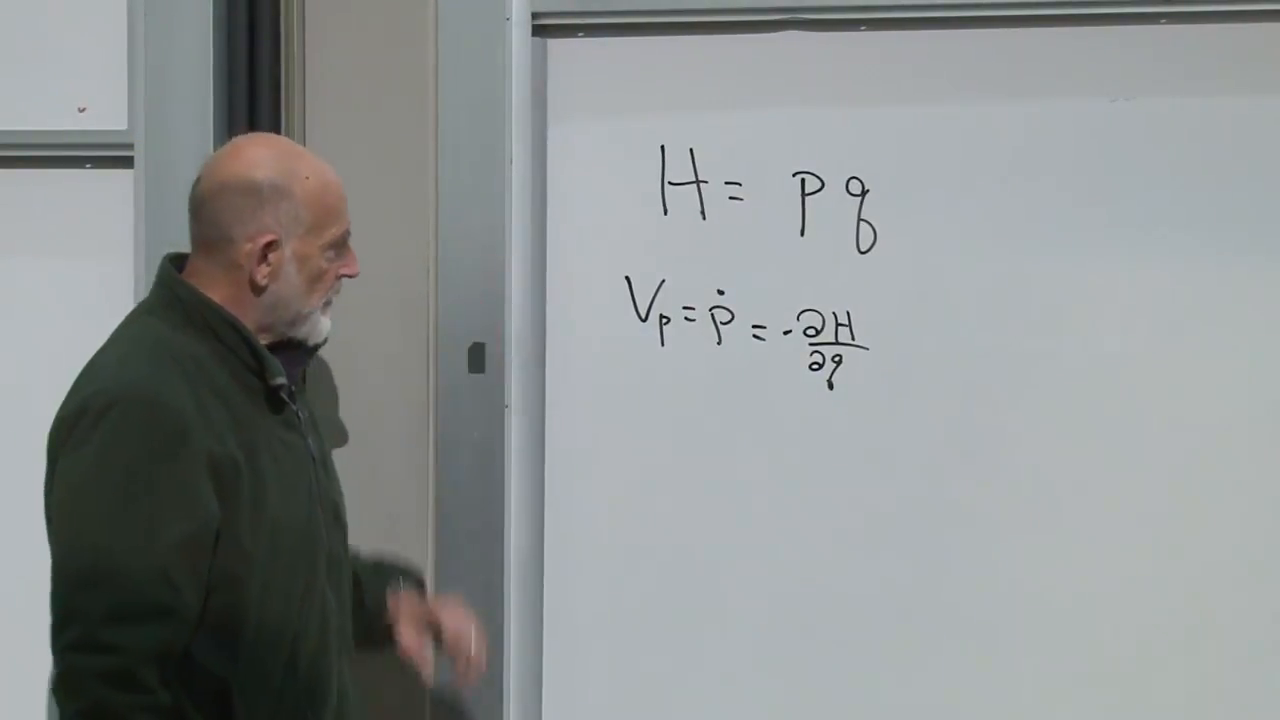
\includegraphics[width=0.82\textwidth]{lecture_07_figure_03.png}
  \caption{\(H=pq\)例子的開頭，以及第一個相空間速度分量。}
  \lectureframe{01:00:11}
\end{figure}

哈密頓方程為
\begin{equation}
  \dot p=-\lambda p,
  \qquad
  \dot q=\lambda q,
  \label{eq:l7-pq-flow}
\end{equation}
其解為
\begin{equation}
  p(t)=p_0e^{-\lambda t},
  \qquad
  q(t)=q_0e^{\lambda t}.
  \label{eq:l7-pq-solutions}
\end{equation}
一個正方形小區域在\(p\)方向上以指數方式縮小，同時在\(q\)方向上以相同因子拉長：
\begin{equation}
  \Delta p(t)\Delta q(t)
  =
  \Delta p(0)\Delta q(0).
  \label{eq:l7-pq-area}
\end{equation}
從局部散度也能驗證這個結果：
\begin{equation}
  \frac{\partial\dot p}{\partial p}
  +\frac{\partial\dot q}{\partial q}
  =-\lambda+\lambda=0.
  \label{eq:l7-pq-divergence}
\end{equation}

\begin{figure}[htbp]
  \centering
  \includegraphics[width=0.86\textwidth]{lecture_07_figure_11.png}
  \caption{在\(H=pq\)流作用下，一個緊緻的小區域被拉長成細長條帶，同時保持面積。}
  \lectureframe{01:02:10}
\end{figure}

\begin{classroomqa}
  \audiencequestion{既然\(pq\)的單位是作用量，劉維爾定理是否表示作用量守恆？\lecturetimestamp{01:03:00--01:04:09}}
  \lecturerresponse{不是。這個定理守恆的是相空間體積。對一組正則變數而言，\(dq\,dp\)的單位是作用量；這個量綱特徵也預示了量子力學，因為相空間胞元的測量單位由\(\hbar\)決定。但乘積\(pq\)本身不是哈密頓作用量泛函，也不會只因量綱相同就自動成為角動量。}
\end{classroomqa}

這個例子也顯示角度不一定保持不變。在式~\eqref{eq:l7-pq-solutions}所示的縮放下，兩臂縮放不等的直角十字，其度量形狀會受到剪切，但面積仍保持不變。劉維爾定理是面積或體積守恆定理，不是一般歐幾里得剛體變換定理。

\section{阻尼會產生匯}

為了看出這個定理排除了什麼，考慮阻尼振子的約化方程：
\begin{equation}
  m\ddot x=-kx-c\dot x,
  \qquad c>0.
  \label{eq:l7-damped-newton}
\end{equation}
令\(p=m\dot x\)。則
\begin{equation}
  \dot x=\frac{p}{m},
  \qquad
  \dot p=-kx-\frac{c}{m}p.
  \label{eq:l7-damped-first-order}
\end{equation}
沒有阻尼時，相點會繞著原點作圓周運動。有阻尼時，能量會傳給周圍介質的微觀自由度，軌道則向內螺旋。

\begin{figure}[htbp]
  \centering
  \includegraphics[width=0.84\textwidth]{lecture_07_figure_13.png}
  \caption{阻尼振子方程，以及它在\(x\)-\(p\)平面上的向內螺旋軌跡。}
  \lectureframe{01:13:30}
\end{figure}

這個二維約化流的散度為
\begin{equation}
  \frac{\partial\dot x}{\partial x}
  +\frac{\partial\dot p}{\partial p}
  =
  0-\frac{c}{m}<0.
  \label{eq:l7-damped-divergence}
\end{equation}
每一個有限區域都會收縮。原點是個匯，是離散狀態映射中多個箭頭匯入同一狀態的連續類比。

\begin{figure}[htbp]
  \centering
  \includegraphics[width=0.88\textwidth]{lecture_07_figure_14.png}
  \caption{阻尼相空間中的速度分量，用來導出負散度\(-c/m\)。}
  \lectureframe{01:16:05}
\end{figure}

這並不表示微觀力學違反劉維爾定理。兩個變數\(x,p\)沒有包含數量龐大的環境自由度，而振子的能量正是傳給了這些自由度。即使約化後的\(x,p\)描述呈現收縮，振子與環境合成的較大系統仍可能遵循哈密頓動力學並保持體積。

\begin{classroomqa}
  \audiencequestion{儘管阻尼振子在這個約化相空間中不是哈密頓系統，它仍然由牛頓方程描述嗎？
  \lecturetimestamp{01:20:09--01:21:12}}
  \lecturerresponse{是的。牛頓第二定律\(F=ma\)可以納入根據經驗給定的阻力。初等的拉格朗日描述\(L=T-V\)和哈密頓描述直接適用於保守力；更一般的拉格朗日量也能處理某些依賴速度的力。然而，對孤立的一對\(x,p\)而言，馬可夫型摩擦項描述的是約化後的耗散動力學，而不是封閉的正則哈密頓系統。}
\end{classroomqa}

\begin{classroomqa}
  \audiencequestion{如果阻尼方程能以無限精度反向積分，資訊真的會丟失嗎？
  \lecturetimestamp{01:25:16--01:27:17}}
  \lecturerresponse{在任何有限時間內，理想的微分方程仍有反函數，因此可以用精確資料反向演化。更精確地說，有限的相空間胞元會呈指數收縮。因此，要重建它們過去的狀態，就需要指數級提高精度；到了無限時間，所有軌跡都會趨近匯點。這是最接近離散「選項消失」圖像的連續經典類比，並不表示兩個精確解在有限時間內真的會合而為一。}
\end{classroomqa}

\begin{classroomqa}
  \audiencequestion{向量場能否散度為零，卻不是由哈密頓量導出的？\lecturetimestamp{01:18:21--01:22:34}}
  \lecturerresponse{當然可以。哈密頓形式是散度為零的充分條件，但不是必要條件。任意不可壓縮速度場都可能散度為零，卻不是同一空間上的正則哈密頓場。三維不可壓縮流體的速度場就是課堂上的例子：三個座標本身無法構成正則共軛對。完整的流體力學或許有更精細的無限維哈密頓表述，但這不會改變此處所說的單向蘊含關係。}
\end{classroomqa}

\section{問題進一步揭示的區別}

\begin{classroomqa}
  \audiencequestion{等能面上的運動，與整個相空間體積保持不變有何關係？
  \lecturetimestamp{01:28:47--01:30:41}}
  \lecturerresponse{兩者是哈密頓結構各自帶來的結果。如果\(H\)不顯含時間，每條軌跡都會留在各自的能量面上。一個有限區域可能跨越許多這樣的能量面；劉維爾定理則指出，整個區域的體積保持不變。對諧振子而言，這個區域的形狀也會保持不變，因為其流動是剛性旋轉。而\(H=pq\)的區域只保持面積，不保持形狀。}
\end{classroomqa}

\begin{classroomqa}
  \audiencequestion{機械功在哈密頓描述中扮演什麼角色？\lecturetimestamp{01:30:44--01:32:57}}
  \lecturerresponse{功描述能量如何穿越所選定的系統邊界。外部作用者可以舉起重物或改變參數，藉此改變子系統的能量；子系統獲得的能量，正是作用者失去的能量。如果把雙方都納入同一個封閉模型，焦點就回到總能量守恆，以及子系統之間的能量交換。}
\end{classroomqa}

\begin{classroomqa}
  \audiencequestion{體積保持不變，也代表拓撲和角度保持不變嗎？\lecturetimestamp{01:33:00--01:33:37}}
  \lecturerresponse{光滑的有限時間哈密頓流會保持拓撲，因為它是可逆的連續形變。但它通常不會保持歐幾里得角度或形狀。諧振子的剛性旋轉確實會保持角度和形狀，而\(H=pq\)的拉伸則說明了這為何只是特例。}
\end{classroomqa}

\begin{classroomqa}
  \audiencequestion{省略勒讓德變換，是因為它沒有物理意義嗎？\lecturetimestamp{01:33:43--01:34:48}}
  \lecturerresponse{不是。勒讓德變換很有用，它把速度描述轉換為動量描述，並在映射正則時導出\(H=\sum_i p_i\dot q_i-L\)。即使沒有特別強調正式名稱，這個構造也已經反覆用過；只是目前這個定理不需要完整的一般理論。}
\end{classroomqa}

\section{泊松括號：進一步的簡化}

最後幾分鐘回到歷史主題。十九世紀的力學一再尋找簡潔的結構，將表面上不同的系統連結起來---力學與幾何光學、粒子與光線、經典軌跡與波動描述。泊松括號也是這類結構之一，在量子力學中尤其重要。

令\(F(q,p)\)為相空間上的任意函數。它可以是座標、動量、乘積\(qp\)，或角動量。沿著運動，其時間變化率為\begin{equation}
  \frac{dF}{dt}
  =
  \sum_i\left(
    \frac{\partial F}{\partial q_i}\dot q_i
    +\frac{\partial F}{\partial p_i}\dot p_i
  \right).
  \label{eq:l7-f-time-derivative}
\end{equation}
代入哈密頓方程：
\begin{equation}
  \frac{dF}{dt}
  =
  \sum_i\left(
    \frac{\partial F}{\partial q_i}
    \frac{\partial H}{\partial p_i}
    -
    \frac{\partial F}{\partial p_i}
    \frac{\partial H}{\partial q_i}
  \right).
  \label{eq:l7-f-hamiltonian-derivative}
\end{equation}

\begin{figure}[htbp]
  \centering
  \includegraphics[width=0.88\textwidth]{lecture_07_figure_15.png}
  \caption{一般相空間函數\(F(q,p)\)的時間導數所遵循的鏈鎖律。}
  \lectureframe{01:42:40}
\end{figure}

這個反覆出現的反對稱組合值得有個名稱。對任意兩個函數\(F\)和\(G\)，將它們的泊松括號定義為
\begin{equation}
  \boxed{
  \{F,G\}
  =
  \sum_i\left(
    \frac{\partial F}{\partial q_i}
    \frac{\partial G}{\partial p_i}
    -
    \frac{\partial F}{\partial p_i}
    \frac{\partial G}{\partial q_i}
  \right).}
  \label{eq:l7-poisson-bracket}
\end{equation}

\begin{figure}[htbp]
  \centering
  \includegraphics[width=0.86\textwidth]{lecture_07_figure_16.png}
  \caption{由兩個函數的導數構成的組合，提升為泊松括號。}
  \lectureframe{01:44:15}
\end{figure}

式~\eqref{eq:l7-f-hamiltonian-derivative}可改寫為
\begin{equation}
  \boxed{\frac{dF}{dt}=\{F,H\}.}
  \label{eq:l7-hamiltonian-poisson-evolution}
\end{equation}
如果\(F\)還顯含時間，則再加上\(\partial F/\partial t\)。令\(F=q_i\)或\(F=p_i\)，即可得到哈密頓的兩個方程，因此式~\eqref{eq:l7-hamiltonian-poisson-evolution}以簡潔形式表達了完整的動力學。

記號總是可以人為地簡化---例如，可以把許多方程各自平方後相加，再稱所得結果為一個方程。這麼做只會隱藏結構，而非揭示結構。泊松括號之所以有用，恰恰是因為它的代數能整理時間演化、守恆量與對稱性。下一步要發展這套代數，再將它用於角動量；角動量的結構在經典力學與量子理論中都至關重要。

\section{可逆性的連續意義}

現在可以完整陳述這一連串想法。當哈密頓量不顯含時間時，哈密頓方程會使\(H\)保持不變，因此每條軌跡都留在等能超曲面上。同一組方程也為相空間中的每一點指定一個速度。由於混合偏導數會兩兩抵消，這個速度場的散度為零。因此，一整個可能狀態區域的正則體積會保持不變。

這就是「一條軌跡進入、一條軌跡離開」的連續版本。形狀和角度都可能改變，相鄰軌跡也可能大幅分離。在光滑且封閉的哈密頓描述中，不可能發生的是：將有限的一組可能狀態壓縮到更小的相空間體積。\(H=pq\)流展示了系統可以拉伸；約化後的阻尼振子則展示了一旦不再滿足哈密頓條件，就會出現匯點。接著，泊松括號將同一套動力學濃縮成一個陳述：哈密頓量生成所有時間導數。